% compile with XeLaTeX
% this template was created by salim bou 
\documentclass[dvipsnames,mathserif]{beamer}
\mode<presentation>
\usepackage{tikz}
\usepackage{pgfplots}
\pgfplotsset{compat=1.18}
\usetikzlibrary{calc}
\usepackage{listings}
\usepackage{xcolor}
\usepackage{arabtex}
\usepackage{mathtools}
 \usepackage[LAE,T1]{fontenc}
%\usepackage[arabic,french,english]{babel}
 
\usepackage{verbatim}

\usetikzlibrary{arrows,shapes,backgrounds}

 \newcommand{\rtx}[1]{\textcolor{red}{#1}}
 
\newcommand{\fr}{\selectlanguage{french}}

\newcommand{\bltx}[1]{\textcolor{blue}{#1}}
\newcommand{\grtx}[1]{\textcolor{green}{#1}}
\newcommand{\blcommand}[2]{\bltx{\bf$\backslash$#1}\{\bf #2\}}
\newcommand{\grcommand}[1]{\grtx{\bf #1}}
%--------------------------------------------------------------
\newcommand{\sncommand}[1]{\bltx{\bf#1$\backslash$}}
\newcommand{\dbcommand}[2]{\{\bf #2\}\bltx{\bf#1$\backslash$}}

\newcommand{\opcommand}[3]{\{\bf #3\}[\grtx{\bf #2}]\bltx{\bf#1$\backslash$}}
\newcommand{\opcommandtwo}[3]{\{\bf #3\}[#2]\bltx{\bf#1$\backslash$}}
%------------------------------------------------------------
\newenvironment{mycode}
    {%\RTListe
    \begin{center}
    \begin{tabular}{|p{0.5\textwidth}|}
    \hline
    \begin{flushright}
    }
    {
    \end{flushright}
    \\\hline
    \end{tabular} 
    \end{center}
    }
 
\newcommand{\gfcb}[1]{%
    \fcolorbox{white}{gray!10!}{\quad\strut #1\quad}
    } % gfcb := gray fcolorbox
\newcommand{\cop}[1]{%
    \ensuremath{\quad\longrightarrow\quad #1}
    \gfcb{\texttt{\detokenize{#1}}} 
    %\ensuremath{\quad\longrightarrow\quad #1}
    } % cop := code output

\usepackage{hyperref}
\newcommand*{\email}[1]{%
    \normalsize\href{mailto:#1}{#1}\par
}
\usepackage{polyglossia}
\setdefaultlanguage[numerals=maghrib,locale=algeria]{arabic} % locale=mashriq, libya, algeria, tunisia, morocco, or mauritania  for names of months in \date 
\setotherlanguage{english}
\newfontfamily\arabicfont[Script=Arabic]{Lateef}
\newfontfamily\arabicfontsf[Script=Arabic]{Lateef}

%\usetheme{Madrid}
\usetheme{modprogressbarMAHER}
%\usecolortheme{crane}
\usetikzlibrary{fadings, backgrounds}
\tikzfading[name=fade out, inner color=transparent!100, outer color=transparent!40]
\tikzfading[name=fade in, inner color=transparent!100, outer color=transparent!0]
%\usetikzlibrary{mindmap}
\usetikzlibrary{shadows}
\usetikzlibrary{shapes,arrows,positioning,automata,backgrounds,calc,er,patterns}

\usepackage{tikz-feynman}

\tikzfeynmanset{compat=1.0.0}
\usetikzlibrary{decorations.pathmorphing, patterns,shapes}

\usepackage[beamer]{hf-tikz}
 
\usetikzlibrary{overlay-beamer-styles}
\tikzset{
	highlight on/.style={alt={#1{fill=red!80!black,color=red!80!black}{fill=gray!30!white,color=gray!30!white}}},
}

%\tikzset{
%	basic/.style  = {draw, text width=2cm, drop shadow, font=\sffamily, rectangle},
%	root/.style   = {basic, thin, align=center,
%		fill=gray!45},
%	level 2/.style = {basic, thin,align=center, fill=gray!30,
%		text width=8em},
%	level 3/.style = {basic, thin, align=left, fill=gray!20, text width=6.5em}
%}
 \tikzset{
 	basic/.style  = {draw, text width=4cm, drop shadow, font=\sffamily, rectangle},
 	root/.style   = {basic, rounded corners=2pt, thin, align=center,
 		fill=green!30},
 	level 2/.style = {basic, rounded corners=3pt, thin,align=center, fill=green!60,
 		text width=10em},
 	level 3/.style = {basic, thin, align=left, fill=pink!60, text width=7.8em}
 }
 
\tikzset{
	pivot/.style={
		draw, 
		regular polygon, 
		regular polygon sides = 3, 
		fill = red, 
		node distance = 1cm, 
		minimum height = 2em,
		at = {(0,0)}
	}
}
% for RTL liste
\makeatletter
\newcommand{\RTListe}{\raggedleft\rightskip\leftm}
\newcommand{\leftm}{\@totalleftmargin}
\makeatother



% RTL frame title
\setbeamertemplate{frametitle}
{\vspace*{-1mm}
  \nointerlineskip
    \begin{beamercolorbox}[sep=0.3cm,ht=2.2em,wd=\paperwidth]{frametitle}
        \vbox{}\vskip-2ex%
        \strut\hskip1ex\insertframetitle\strut
        \vskip-0.8ex%
    \end{beamercolorbox}
}


% align subsection in toc
\makeatletter
\setbeamertemplate{subsection in toc}
{\leavevmode\rightskip=5ex%
  \llap{\raise0.1ex\beamer@usesphere{subsection number projected}{bigsphere}\kern1ex}%
  \inserttocsubsection\par%
}
\makeatother

% RTL triangle for itemize
\setbeamertemplate{itemize item}{\scriptsize\raise1.25pt\hbox{\donotcoloroutermaths$\blacktriangleleft$}} 

%\setbeamertemplate{itemize item}{\rule{4pt}{4pt}}

\defbeamertemplate{enumerate item}{square2}
{\LR{
    %
    \hbox{%
    \usebeamerfont*{item projected}%
    \usebeamercolor[bg]{item projected}%
    \vrule width2.25ex height1.85ex depth.4ex%
    \hskip-2.25ex%
    \hbox to2.25ex{%
      \hfil%
      {\color{fg}\insertenumlabel}%
      \hfil}%
  }%
}}

\setbeamertemplate{enumerate item}[square2]

\setbeamertemplate{navigation symbols}{}

%%%%%%%%%%%%%%%%%%%%%%%%%%%%[ blocks ]%%%%%%%%%%%%%%%%%%%%%%%%%%%%%%%%%%%%
\newenvironment<>{problock}[1]{%
	\begin{actionenv}#2%
		\def\insertblocktitle{#1}%
		\par%
		\mode<presentation>{%
			%\setbeamercolor{block title}{fg=white,bg=blue!48!black}
			\setbeamercolor{block body}{fg=white,bg=pbblue}
			%  \setbeamercolor{itemize item}{fg=orange!20!black}
			%  \setbeamertemplate{itemize item}[triangle]
		}%
		\usebeamertemplate{block begin}}
	{\par\usebeamertemplate{block end}\end{actionenv}}
 
%=========================================================================
\begin{document}
 
\title{كورس مكثف لتعلم الLaTeX على محرر Overleaf}
\logo{
\includegraphics[width=0.5cm]{figs/sudan_logo.png}}
\author[محمد ماهر عبد الرحيم محمد]{         \href{https://www.facebook.com/mohammedmaher8932/}{\it{محمد ماهر عبد الرحيم محمد}}  }
\institute{
    \href{https://www.facebook.com/groups/651884204836245}{\Large{ملتقى الفيزيائيين السودانيين}} 
}
\vspace{-2cm}
%\date{\today}
%\affil{\it{The Insider Researcher Group, Khartoum, Sudan}\\

\date{17/02/2023}
%---------------------------------------------------------------------------
%---------------------------------------------------------------------------
\begin{frame}

    \begin{center}
        \maketitle
        
\includegraphics[scale=0.1]{figs/sfp.jpg}
        
\includegraphics[scale=0.2]{figs/online-editor-2.png}
        
\includegraphics[scale=0.1]{figs/sfp.jpg}
    \end{center}

\end{frame}
%---------------------------------------------------------------------------
%---------------------------------------------------------------------------

%============================================================================
\begin{frame}{التعريف ببرنامج الدورة}

    \begin{itemize}\RTListe
     \item
    اليوم الأول: مدخل إلى \LaTeX{}
        \begin{itemize}\RTListe
            \item مقدمة عن \LaTeX{} واستخداماته
            \item هيكل الوثيقة الأساسية وتنسيقها
            \item إنشاء أقسام وفقرات وفواصل أسطر
            \item  التنسيق الرياضي الأساسي
        \end{itemize}
    \item اليوم الثاني: تنسيق \LaTeX{} المتقدم
        \begin{itemize}\RTListe
            \item  عمل الجداول والأشكال
            \item  تنسيق رياضي متقدم
            \item إنشاء الببليوجرافيات والاستشهادات
        \end{itemize}
    \item اليوم الثالث: أفضل الممارسات والتطبيقات
        \begin{itemize}\RTListe
            \item إنشاء وحدات ماكرو و بيئات مخصصة
            \item إنشاء عروض تقديمية باستخدام \LaTeX{}
        \end{itemize}
    \end{itemize}

\end{frame}
%==========================================================
%////////////////////////////////////////////////////////////////////////////////////
%============================================================================
\begin{frame}[plain]
	\addtocounter{framenumber}{-1}
	\begin{problock}{}
		\LARGE
		\vfill
		\centerline{\bf \textcolor{red}{\bf اليوم الأول: الأساسيات}}		
		\vfill
	\end{problock}
 
\end{frame}
%==========================================================
\begin{frame}{المحتويات}
    \tableofcontents
\end{frame}
%=========================================================
\section{ما هو \LaTeX\ ولماذ نحتاجه  }
%-------------------------------
\begin{frame}{ما هو \LaTeX\ ولماذ نحتاجه  }

    \begin{exampleblock}{\LaTeX{}}
    هو نظام إعداد الوثائق و المستندات يستخدم في كتابة (االأوراق العلمية، البحوث، التقارير و الكتب ...) عالية الجودة بدقة واتساق كبيرين
    \end{exampleblock}
    \begin{center}
        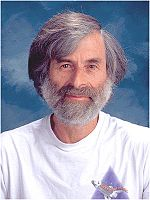
\includegraphics[scale=0.4]{figs/Lamport.png} 
        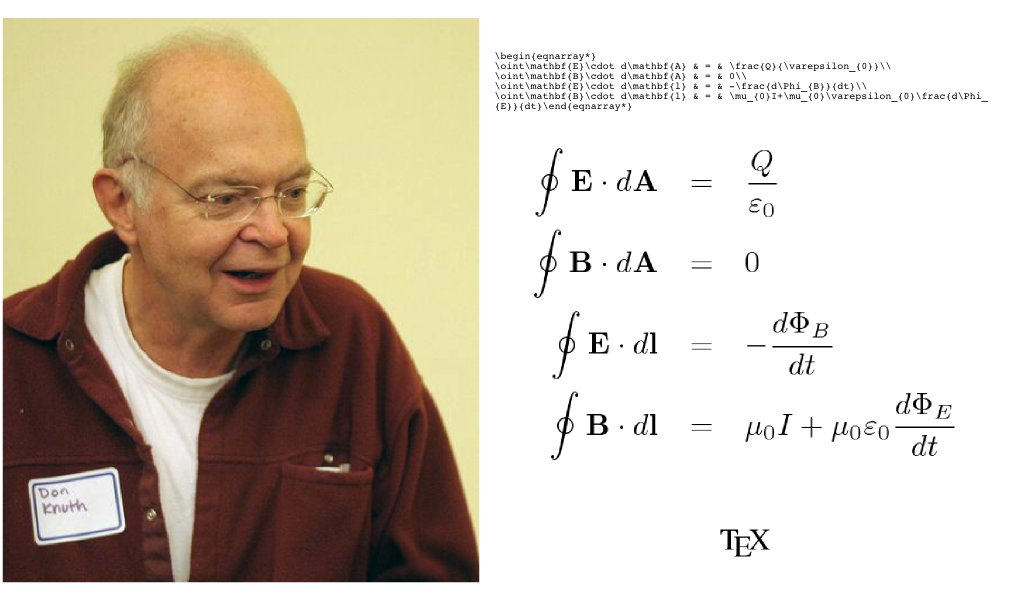
\includegraphics[scale=0.2]{figs/fig_knuth_tex.jpg} 
    \end{center}
 
\end{frame}
%==============================================
\begin{frame}{ كيف يعمل ال\LaTeX{}}
   
    \bc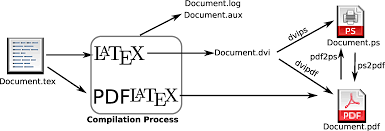
\includegraphics[scale=0.5]{figs/comp.png}\ec
    \begin{center} 
        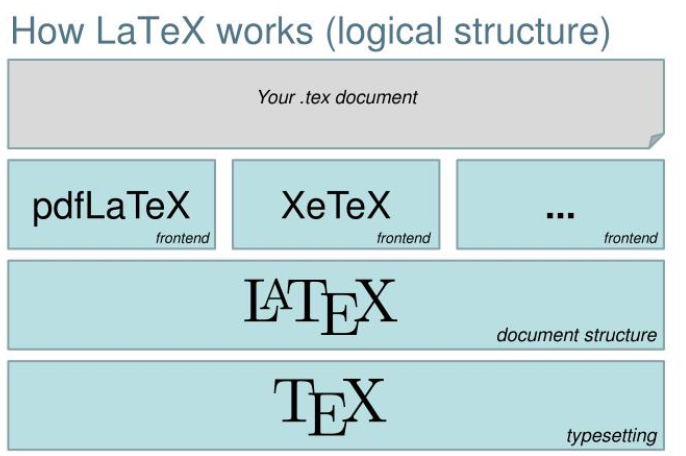
\includegraphics[scale=0.25]{figs/howLW.png}
    \end{center}

\end{frame}
%==============================================
\begin{frame}[shrink=15]\frametitle{المميزات}
 
المميزات:
    \begin{itemize}\RTListe
        \item يوفر التحكم الكامل في التنسيق الصفحة، مما يجعل النصوص الأكاديمية والعلمية جيدة الشكل ولطيفة المشاهدة.
        \item يجعل العمل مع الجداول والصور و الفقرات النصية سهلاً ويسهل التنسيق الجانبي.
        \item يوفر الدعم الكامل لللغات بما فيهم العربية.
        \item يجعل التعامل مع الإشارات المرجعية الأكاديمية والأعداد الإحصائية و الجداول سهلاً.
        \item يعطي الملف في شكل PDF او PS جاهزة للطباعة  .
    \end{itemize}
    
    \begin{columns}
        \column{0.7\textwidth}
        \centering
            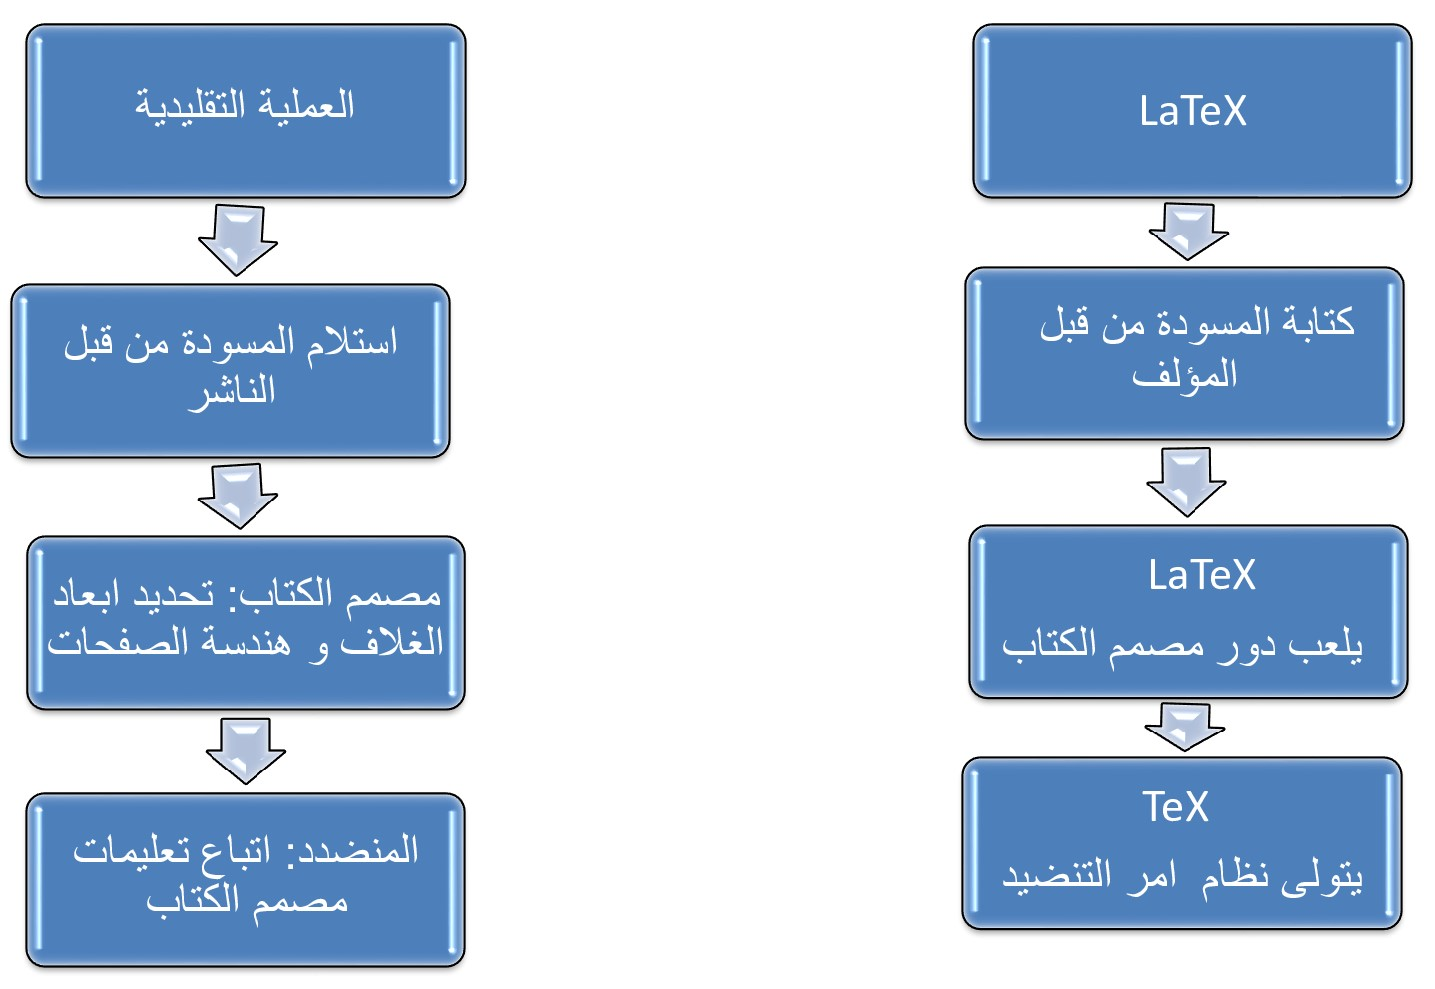
\includegraphics[scale=0.15]{figs/process.jpg}
            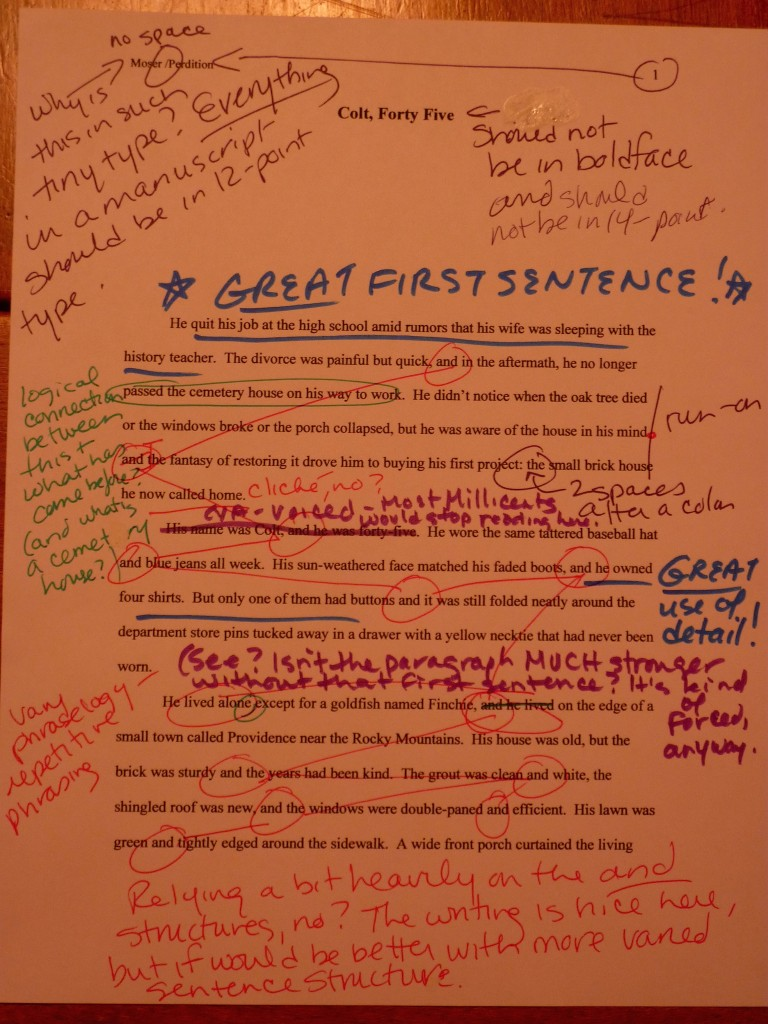
\includegraphics[scale=0.1]{figs/mprocess.jpg}
        %%%%%%
        \column{0.3\textwidth}
        \centering
            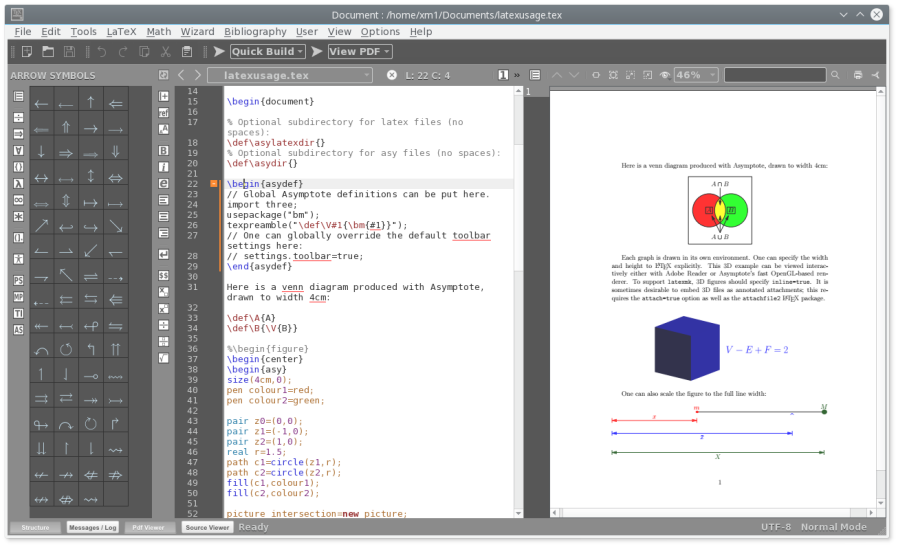
\includegraphics[scale=0.2]{figs/latexprocess.png}
    \end{columns}  

\end{frame}
%==============================================
\begin{frame}[shrink=25]{مقارنة مع معالجات النصوص التقليدية}
 
        \begin{center}
              \begin{tabular}{|c|c|c|}
        \hline
            \textbf{\large المعيار} & \textbf{\large محررات النصوص التقليدية} & \textbf{\large\LaTeX} \\
            \hline\hline
            جودة المخرجات & تعتمد على مهارة المستخدم & الجودة العالية للمخرجات مضبوطة مسبقا بغض النظر عن مهارة المستخدم\\
            \hline
            ضخامة المحتوى & ينهار النظام و يصبح غير مستقر & مستقر و سريع و ثابت بغض النظر عن الحجم المحتوى \\
            \hline
            المراجع و الاستشهادات & تتطلب برامج خارجية & يتم التعامل معاها باحترافية كميزة مدمجة \\
            \hline
            تقسيم العمل الى ملفات منفصلة & لا يوجد حل عملي غالبا & متاح \\
             \hline
            الثمن & بعض البرامج مدفوعة & مجاني و سيظل مجاني \\
            \hline
        \end{tabular}      
        \end{center}

  \begin{center}
     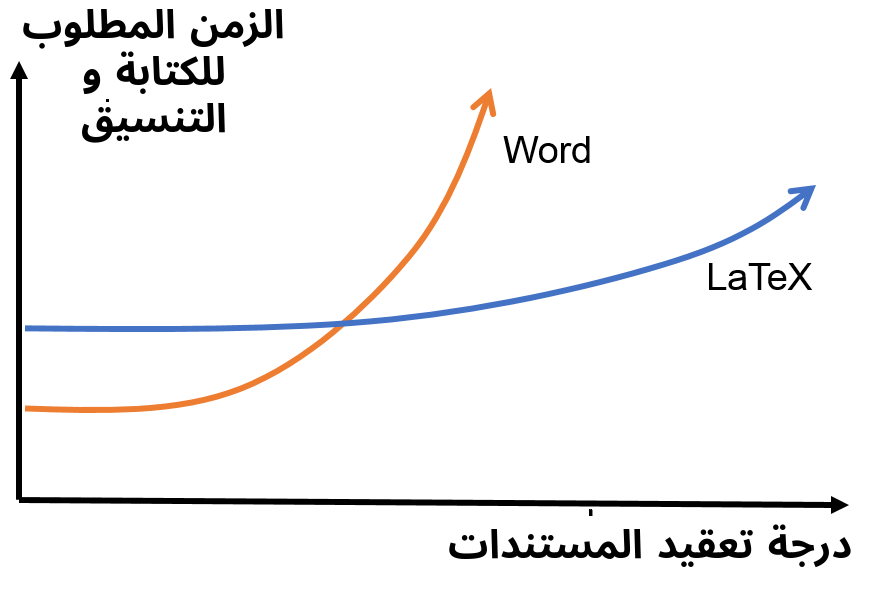
\includegraphics[scale=0.25]{figs/word_vs_latex_1_eng.png}
 \end{center}
\end{frame}
%==============================================
\begin{frame}{محررات نصوص ال\LaTeX{}}
\bc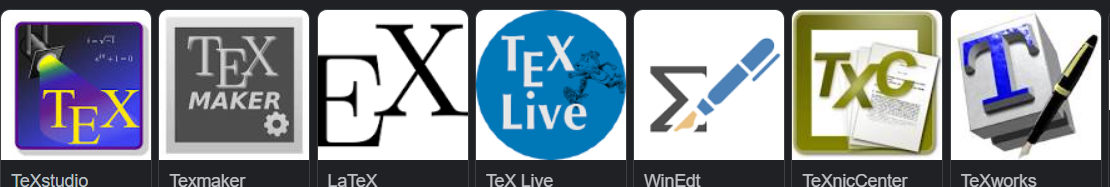
\includegraphics[scale=0.3]{figs/editors.png}\ec
\newline
\underline{من الضروري وجود: }
    \begin{itemize}\RTListe
        \item 
    \href{https://miktex.org/download}{\textcolor{blue}{MiKTeX}} لنظام التشغيل Windows
    \item
   \href{https://www.tug.org/texlive/}{\textcolor{blue}{TeX Live}} لنظام التشغيل Linux والأنظمة الأخرى المشابهة لـ UNIX
    \item
    إعادة توزيع \href{https://www.tug.org/mactex/}{\textcolor{blue}{MacTeX}} لـ TeX Live لنظام التشغيل macOS
    \item
    \href{https://www.tug.org/tetex/}{\textcolor{blue}{teTeX}} لنظام التشغيل Linux والأنظمة الأخرى المشابهة لـ UNIX ؛ لم يعد يتم صيانته بنشاط الآن
    يعتمد proTeXt على MiKTeX
    \end{itemize}
\end{frame}
%==============================================
\begin{frame}[shrink=15]{منصة Overleaf}
\begin{itemize}\RTListe
    \item  \href{http://www.overleaf.com/}{\textcolor{green}{\bf :Overleaf}} محرر \LaTeX{} تعاوني يسمح للمستخدمين
لإنشاء وتحرير ومشاركة المستندات المكتوبة بلغة لاتك.
\end{itemize}
\begin{center}
    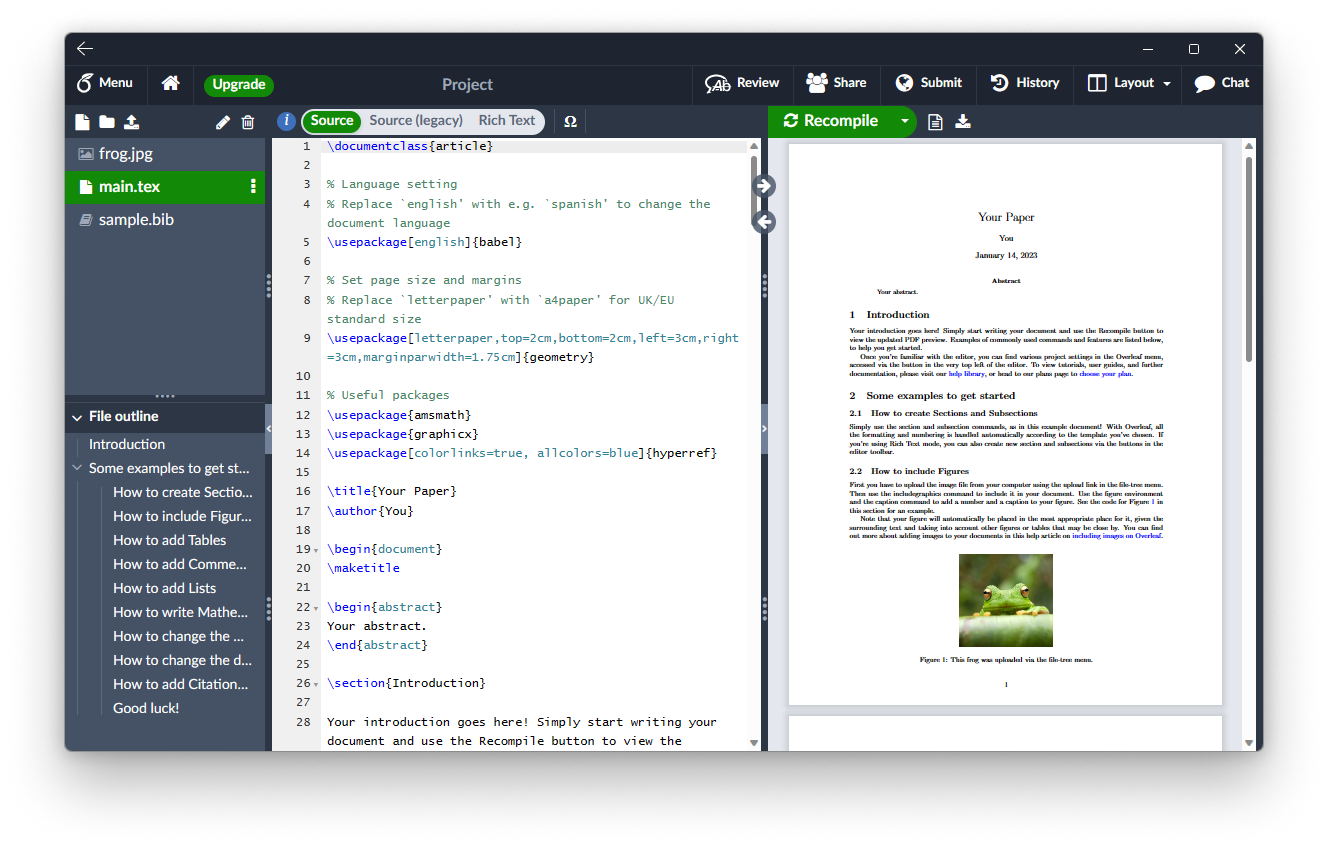
\includegraphics[scale=0.20]{figs/Screenshot_of_Overleaf.png}
\end{center}
\vspace{-1cm}
\begin{itemize}\RTListe
    \item \textcolor{red}{محرر على الإنترنت}: دون الحاجة إلى تثبيت محلي لـ \LaTeX{}.
    \item
\textcolor{red}{التعاون}: من السهل على الفرق التعاون في مشروع ما.
\item
\textcolor{red}{القوالب}: من السهل على المستخدمين البدء بمشروع جديد.
\item
\textcolor{red}{التكامل مع الخدمات الأخرى}: مزامنة المستندات والوصول إليها من خدمات أخرى
المنصات.
\item
\textcolor{red}{المشاركة والنشر}: الإرسال المباشر.
\end{itemize}
    \href{https://www.overleaf.com/for/universities}{خارطة المؤسسات البحثية و الجامعات التى تستخدم Overleaf}
\end{frame}
%==============================================
\section{الهيكل العام لوثيقة ال\LaTeX }
\begin{frame}[shrink=15]{الهيكل العام لوثيقة ال\LaTeX }
\begin{columns}
    \column{0.6\textwidth}
    \begin{mycode}
    \begin{flushleft}
       \dbcommand{documentclass}{article} \\
         منطقة الديباجة حيث تضم نوع المستند و يكتب فيها الحزم المراد استخدامها والضبط الفني للمخرجات \\
        \dbcommand{begin}{\grtx{document}} \\
        
        متن المستند حيث يُكتب المحتوى النصي للمستند \\
    
        \dbcommand{end}{\grtx{document}} \\
        \end{flushleft}
 \end{mycode}
     \column{0.5\textwidth}
    \begin{itemize}\RTListe
	  		\item الديباجة (Preamble) 
	  	
	  		\begin{itemize}\RTListe
	  			\item صَنْف المستند  class document \newline [ book.. report, article,  ]  
	  			\item حِزْمَ إضافية packages additional
	  		\end{itemize}
	  		
	  		\item مَتْن المستند body Document
	  \end{itemize}
 \end{columns}
 
 	\underline{قواعد عامة}
 \begin{itemize}\RTListe
    \item[\checkmark]  تبدأ الاوامر بوضع شرطة مائلة للخلف($\backslash$) قبل كتابة اول حرف من الأمر
   \\
    علي سبيل \textcolor{red}{المثال}:  \textcolor{red}{tableofcontents$\backslash$}
    \item[\checkmark] بعض الأوامر تحتاج إلى عَامِل لكي يظهر تأثيرها عليهايتم وضعها في اقواس معقوفة
   \\
    \textcolor{red}{مثال}:  \textcolor{red}{\{Ali\}}\textcolor{black}{author$\backslash$}
    \item[\checkmark] بعض الأوامر توفر خيارات إضافية، توضع هذه الخيارات بين اقواس مربعة
    \\
     \textcolor{red}{مثال}:   \textcolor{black}{\{book\}}\textcolor{red}{[a4paper,11pt]}\textcolor{black}{documentclass}\textcolor{blcak}{$\backslash$}.
\end{itemize}
\bc
\includegraphics[scale=0.1]{autodraw 05_02_2023.png}\ec
\end{frame}
%=============================================
\begin{frame}[shrink=20]
\begin{columns}
    \column{0.4\textwidth}
    \bc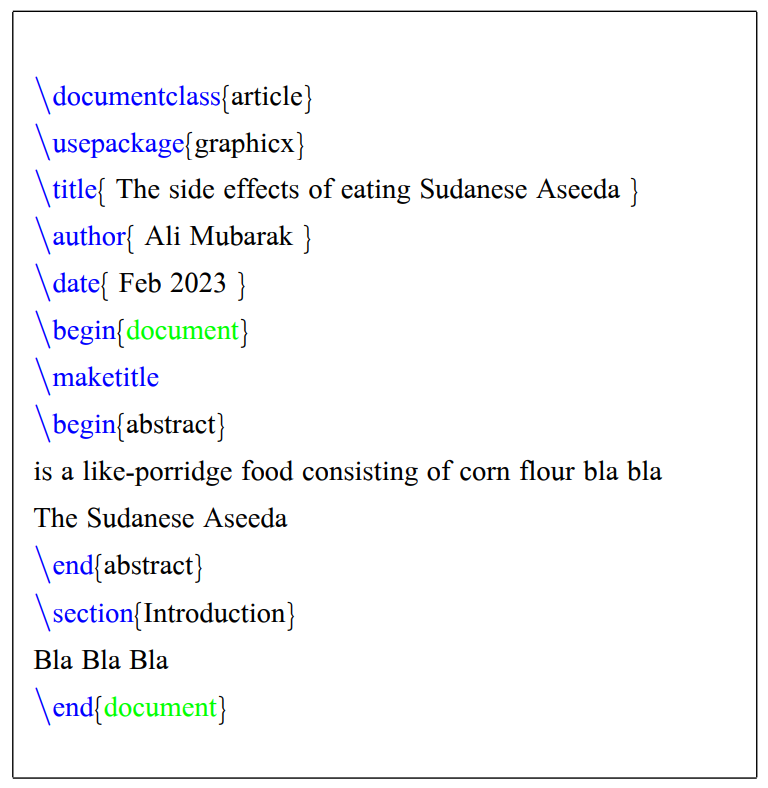
\includegraphics[scale=0.35]{figs/stexample.png}\ec
    \column{0.6\textwidth}
    \bc
\includegraphics[scale=0.8]{figs/aseeda.png}\ec
\end{columns}

\begin{itemize}\RTListe
    \item \textbf{منطقة الديباجة:}
    \begin{itemize}\RTListe
        \item \dbcommand{documentclass}{article}: هنا نقوم بتحديد نوع المستند المراد العمل عليه
        \item  \dbcommand{usepackage}{graphicx}: استدعاء حزمة مطلوبة لاضافة الصور.
        \item \sncommand{title}, \sncommand{author}, \sncommand{date}: العنوان، التاريخ و إسم المؤلف على التوالي.
    \end{itemize}
    \vspace{-0.4cm}
    \item \textbf{منطقة متن المستند:}
     \begin{itemize}\RTListe
        \item
        في اللاتك عموما تسمى المنطقة المحصورة بين أمري \sncommand{begin{}} و \sncommand{end{}} بالبيئة أو المحيط. 
        \item \sncommand{maketitle}: فبدونه لن يظهر اي عنوان او اسم مؤلف او تاريخ او اي معلومة مراد لها الظهور في صفحة العنوان.
        \item \dbcommand{begin}{abstract}\dbcommand{end}{abstract}: البيئة المخصصة لكتابة مستخلص البحث    ،
        \item \dbcommand{section}{Introduction}: الامر المسؤول عن انشاء الاقسام داخل المستند، في هذا المثال قمنا بإنشاء قسم يحمل عنوان مقدمة.
     \end{itemize}
\end{itemize}
\end{frame}
%=============================================
%\begin{frame}
 % \begin{center}
 %     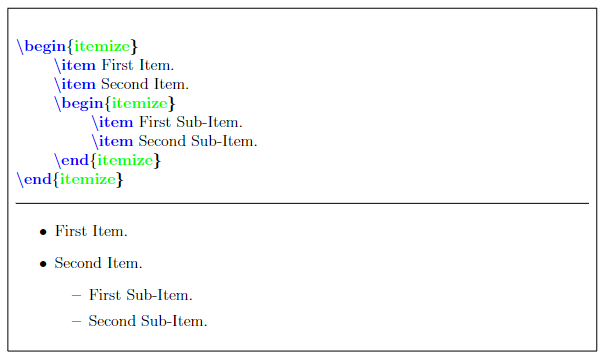
\includegraphics[scale=0.5]{figs/list1.png}
  %    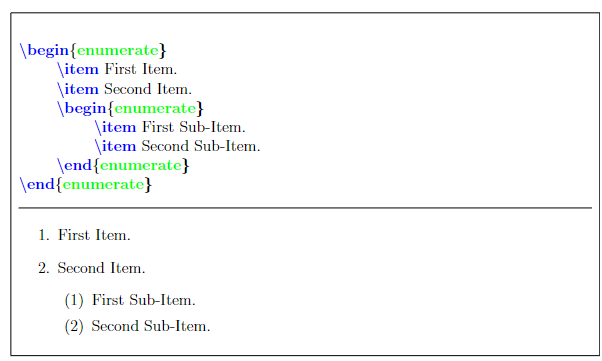
\includegraphics[scale=0.5]{figs/list2.png}
 % \end{center}
%\end{frame}
%==============================================
%\begin{frame}{قم بإنشاء مستندك الأول في  \LaTeX\ }
%  \begin{columns}
%		\column{0.5\textwidth}
%		\begin{center}
%			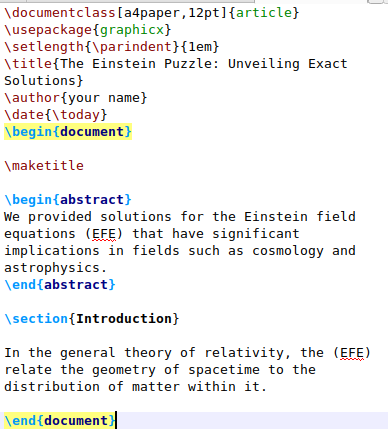
\includegraphics[scale=0.4]{figs/testo}
%		\end{center}
%	\column{0.5\textwidth}
 %
%	  \bc 
\includegraphics[scale=0.16]{figs/outtest} \ec
%	\end{columns} 
%\end{frame}
%==============================================
\begin{frame}[shrink=0]{ نوع المستند }
    \dbcommand{documentclass}{...}
    \begin{itemize}\RTListe
        \item تحدد نوع المستند الذي تعمل به ، وتحميل العديد من الأنماط الافتراضية وتعيين المظهر العام للمستند
    \end{itemize}
    \begin{center}
        \begin{tabular}{|c|c|}
        \hline
         نوع المستند    &  الاستخدام\\
             \hline\hline
          article   &  للمقالات في المجلات العلمية ، والتقارير القصيرة. 
          \\
          \hline
        report  & لتقارير أطول من عدة فصول ، كتب صغيرة ، أطروحات. \\
        \hline
        book  & للكتب \\
          \hline
        \end{tabular}
    \end{center}
    \opcommand{documentclass}{خيار1، خيار2، ...الخ}{نوع المستند}
    \begin{itemize}\RTListe
        \item حجم الخط ( 12pt ، 11pt ، 10pt )
        \item   حجم الورقة و شكلها ( letterpaper ، a5paper ، a4paper )
        \item الأوراق أحادية الوجه ومزدوجة الوجه ( oneside ، twoside )
    \end{itemize}
\end{frame}
%==============================================
\begin{frame}
    \begin{itemize}\RTListe
        \item حجم الخط ( 12pt ، 11pt ، 10pt ) \\
        \bc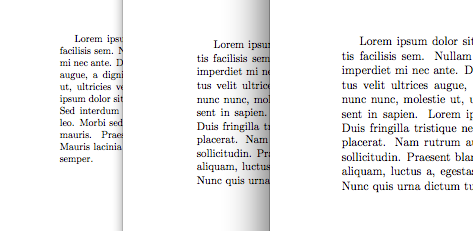
\includegraphics[scale=0.3]{figs/font-size1.png}\ec
        \item   حجم الورقة و شكلها\\
        \bc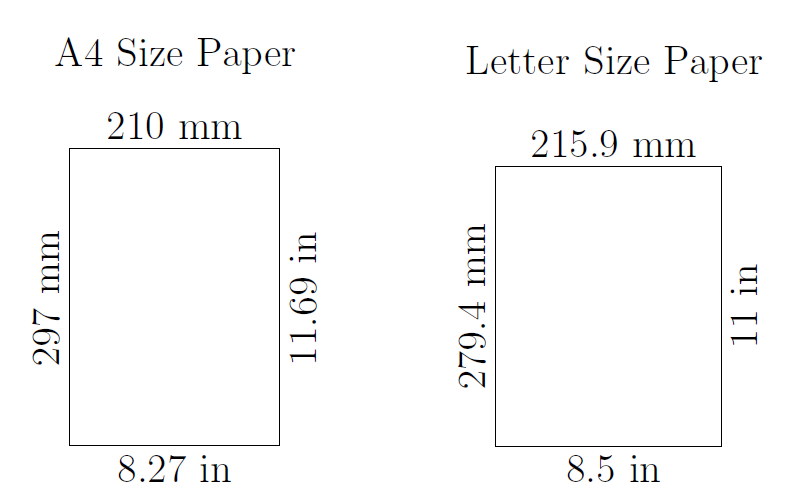
\includegraphics[scale=0.3]{figs/papersize.png}\ec
    \end{itemize}
    
    
\end{frame}
%==============================================
 \begin{frame}{ جزم ال\LaTeX{} }
    \dbcommand{usepackage}{...}
    \begin{itemize}\RTListe
        \item تنقسم بشكل عام إلى فئتين:
        \begin{itemize}\RTListe
            \item الحزم التي تسمح لك بتغيير تخطيط أو هيكل المستند مثل الحزمة geometry 
            \item    الحزم التي تسمح لك بتضمين محتوى جديد أو محسّن المستند tikz latex  
        \end{itemize}
    \end{itemize}
    
\begin{columns}
    \column{0.5\textwidth}
\begin{tikzpicture}
  \pgfplotsset{
    every axis legend/.append style={
      at={(0.5,0)},
      anchor=south,legend columns=2
    }}
  \begin{axis}[unit vector ratio=1 1 1, axis lines=none, view={120}{30}]
		
  % Parte inferior del cilindro
  % Min utiliza el menor valor entre el eje z sin parametrizar y la z parametrizada 
  \addplot3[surf,z buffer=sort,samples=30,colormap/viridis,
    variable=\u, variable y=\v,
    domain=0:360, y domain=0:3]
    ({cos(u)}, {sin(u)},{min(2-y,v)});		

  % Plano parametrizado y+z=2
  \addplot3[surf, z buffer=sort, samples=30,
    variable=\u, variable y=\v,domain=-2:2, y domain=-2:2]({u}, {v},{2-v});

  % Interseccion parametrizada
  \addplot3[color=black,smooth,samples=30,
     variable=\u,domain=0:360,line width=1.25pt]
    ({cos(u)}, {sin(u)},{2-sin(u)});

  % Parte superior del cilindro. Utiliza max tal en la parte inferior
  \addplot3[colormap/viridis,surf,z buffer=sort,samples=30,variable=\u, variable y=\v,
    domain=0:360, y domain=0:4]({cos(u)}, {sin(u)},{max(2-y,v)});
 
  % NOTA: el orden de dibujo de las superficies cambia si se aplica una vista diferente a la 120 30
  \legend{$x^2+y^2=4$,$y+z=2$}
  \end{axis}		
\end{tikzpicture}

%----
\column{0.5\textwidth}
\bc
    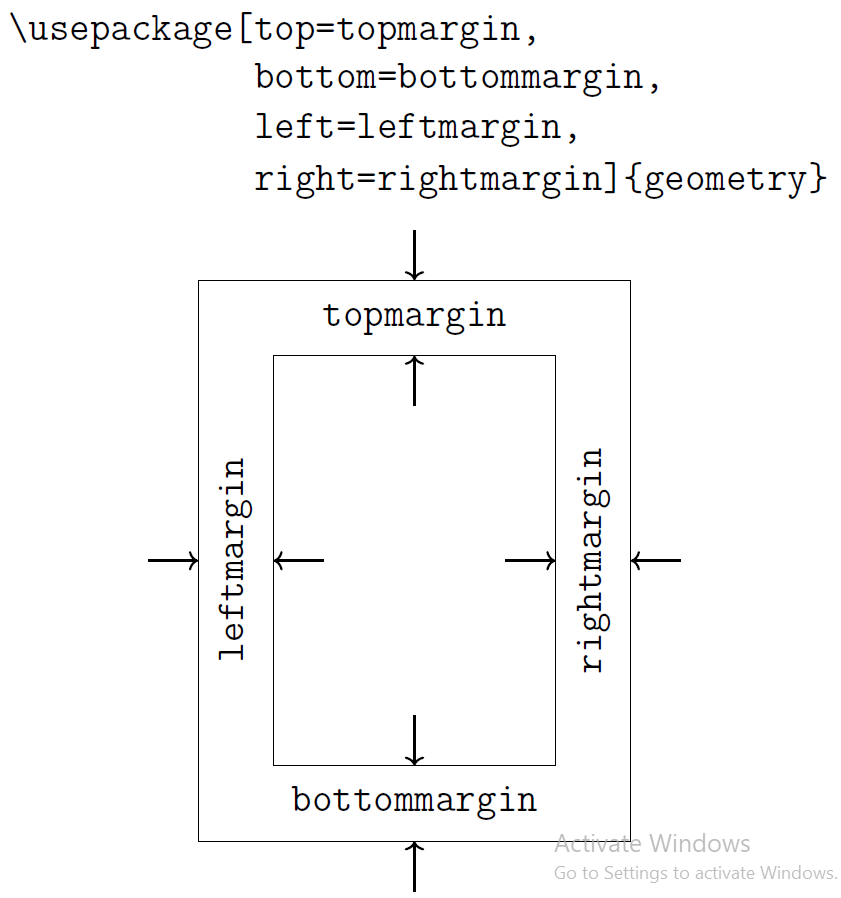
\includegraphics[scale=0.2]{figs/geo.png}
\ec
    
\end{columns}
\end{frame}
%==============================================
\begin{frame}{البيئات في ال\LaTeX{}}
\begin{center}
    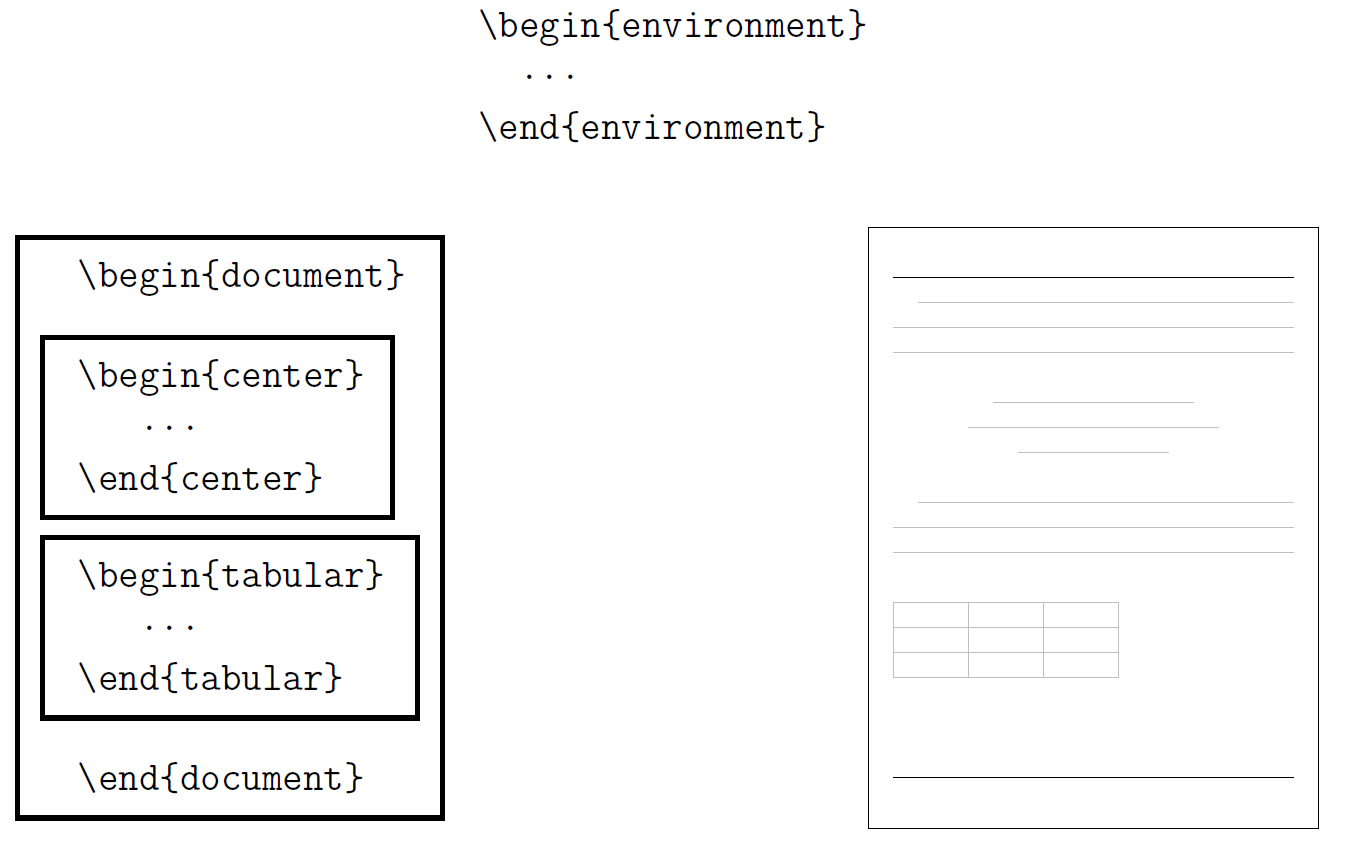
\includegraphics[scale=0.3]{figs/einv.png}
\end{center}
\end{frame}
%==============================================
\begin{frame}
\begin{center}
    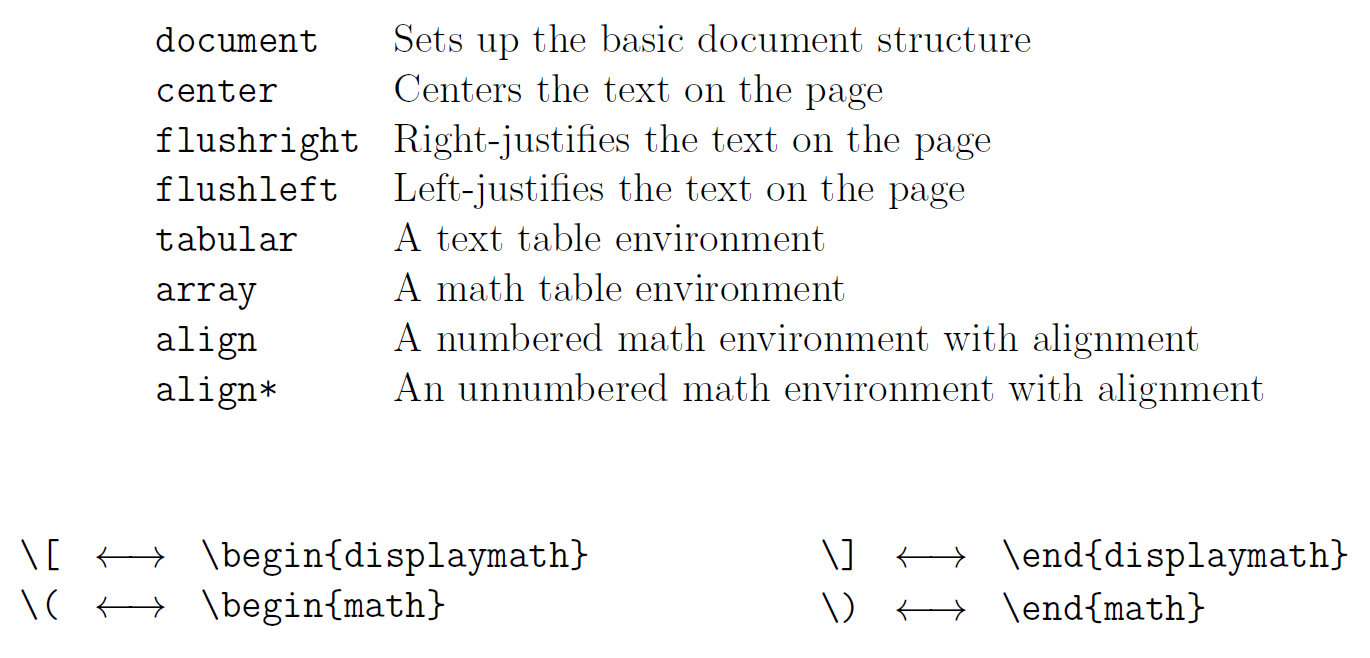
\includegraphics[scale=0.3]{figs/env2.png}
\end{center}
\end{frame}
%==============================================
\section{ (المحتوى) متن المستند}
\begin{frame}{فقرات وأسطر جديدة}
\begin{center}
    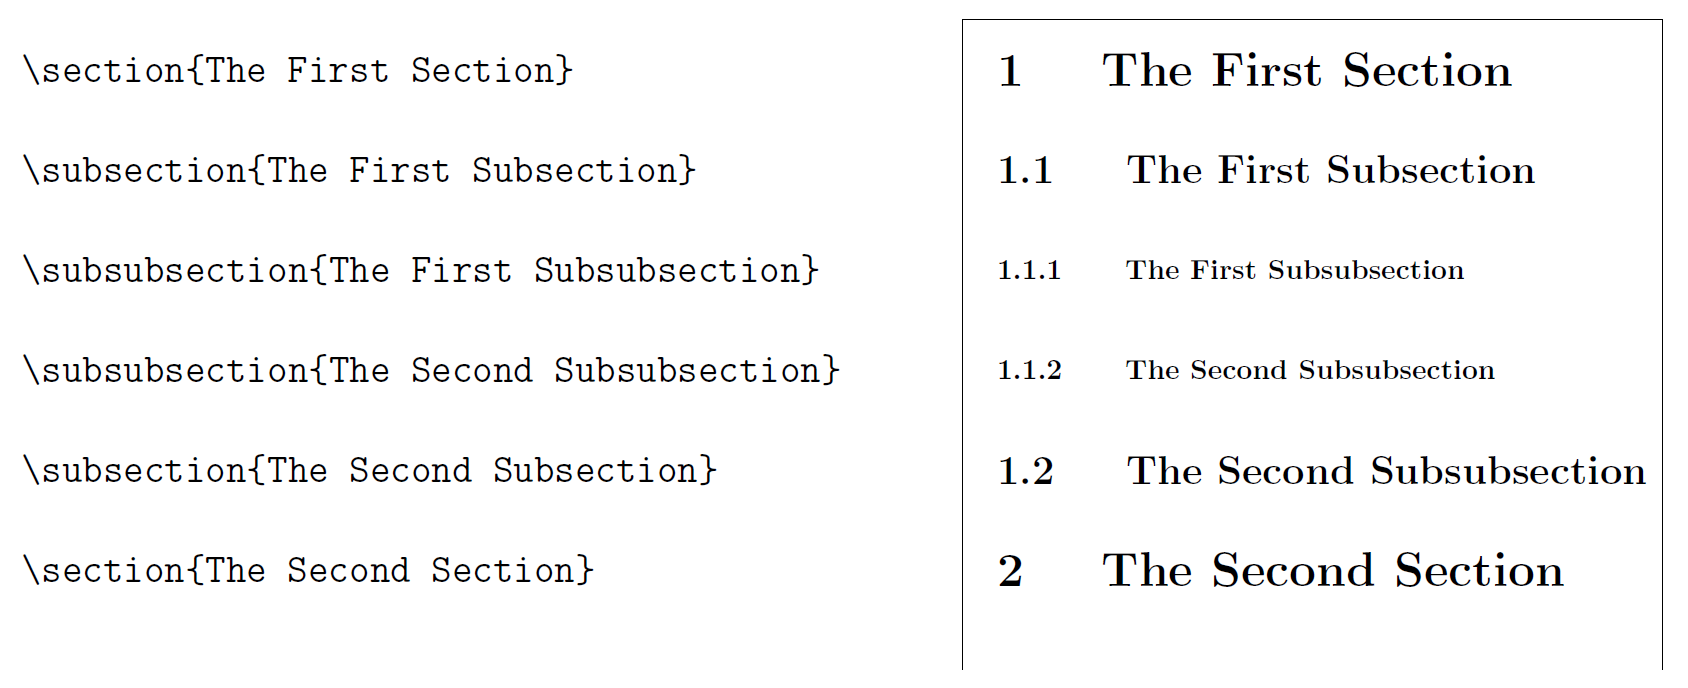
\includegraphics[width=11cm]{figs/sections.png}
\end{center}
\end{frame}
%==============================================
\begin{frame}{المحاذاة}
    \centering
    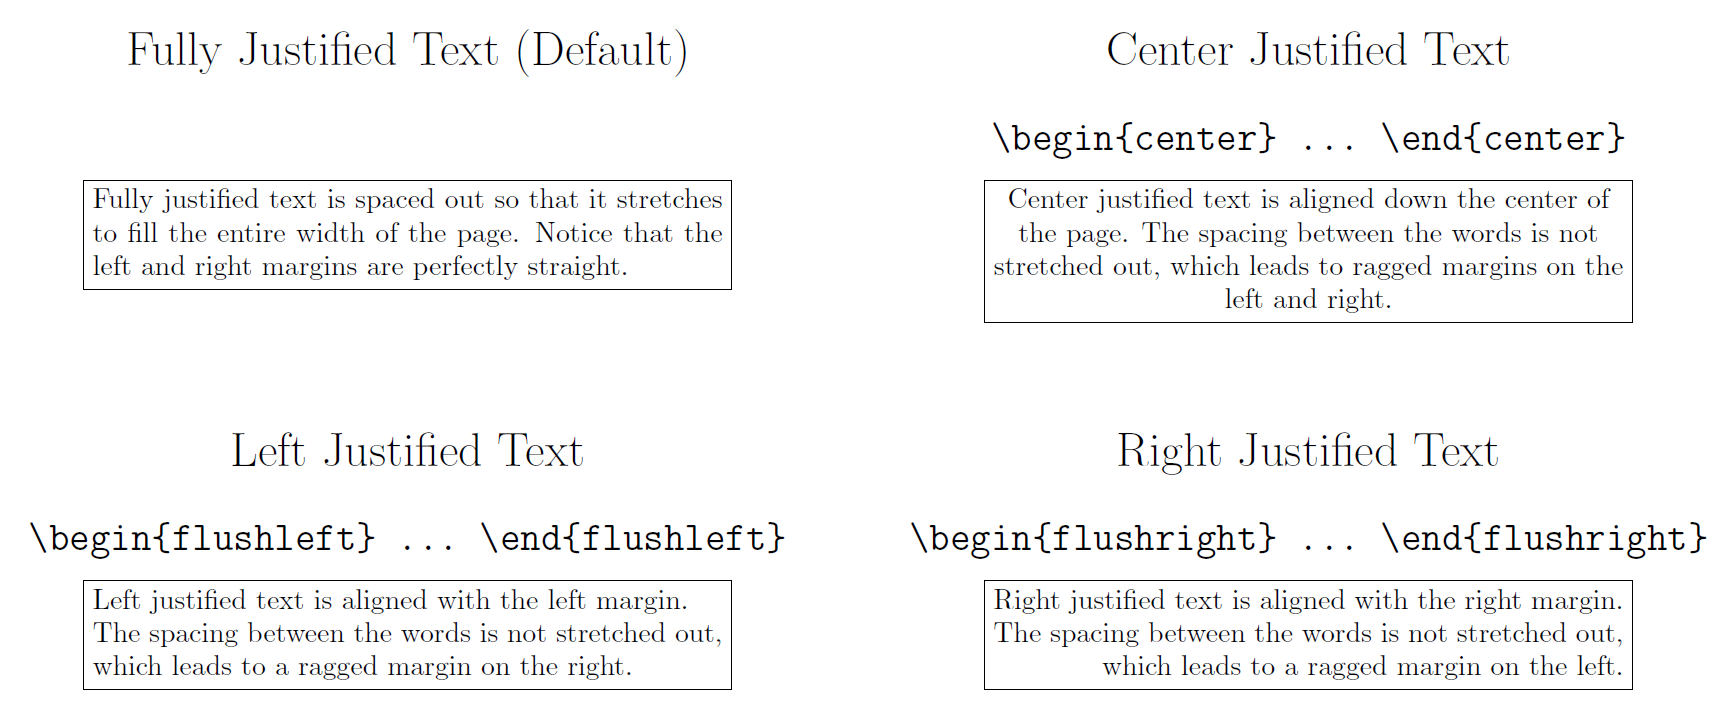
\includegraphics[width=11cm]{figs/paragraph1.png}
\end{frame}
%==============================================
\begin{frame}{الاسطر الجديدة}
    \centering
    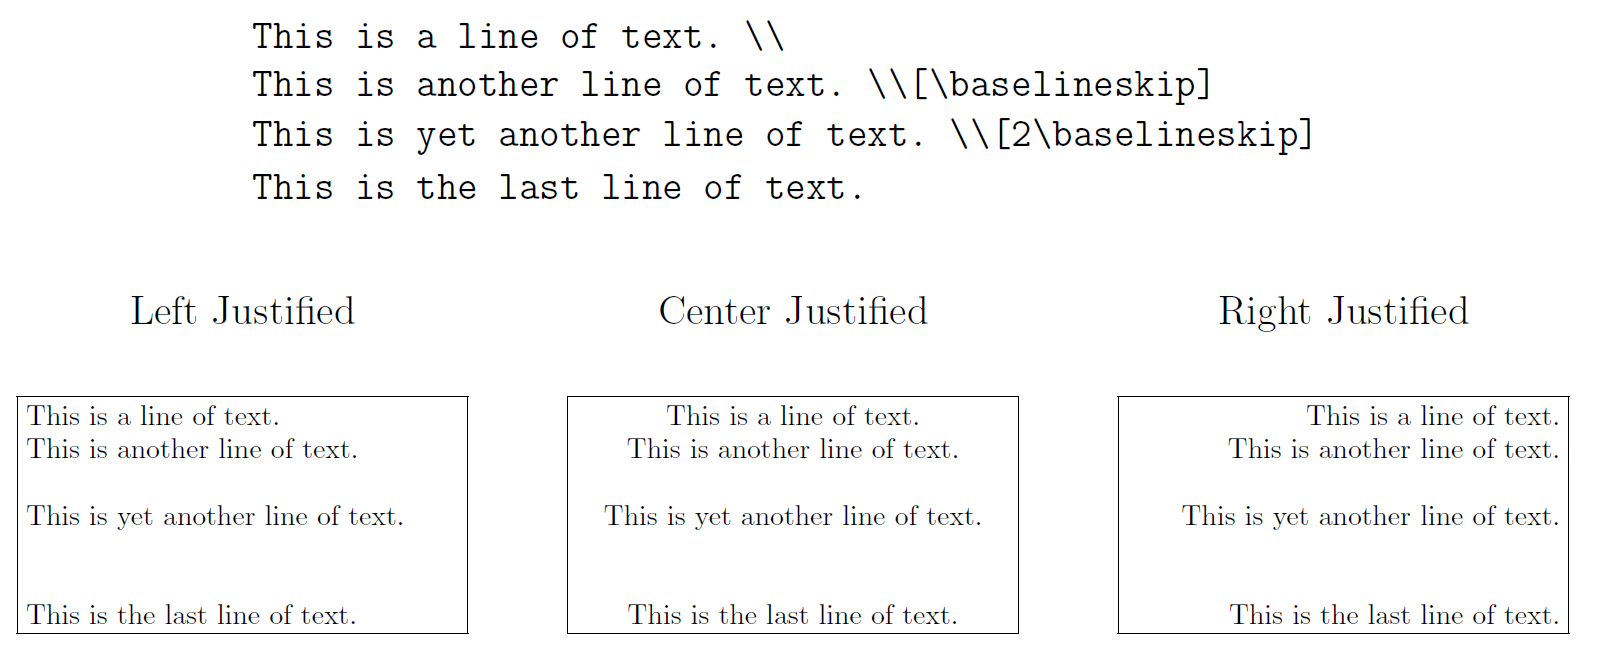
\includegraphics[width=11cm]{figs/paragraph2.png}
\end{frame}
%==============================================
\begin{frame}{القوائم}
\begin{center}
    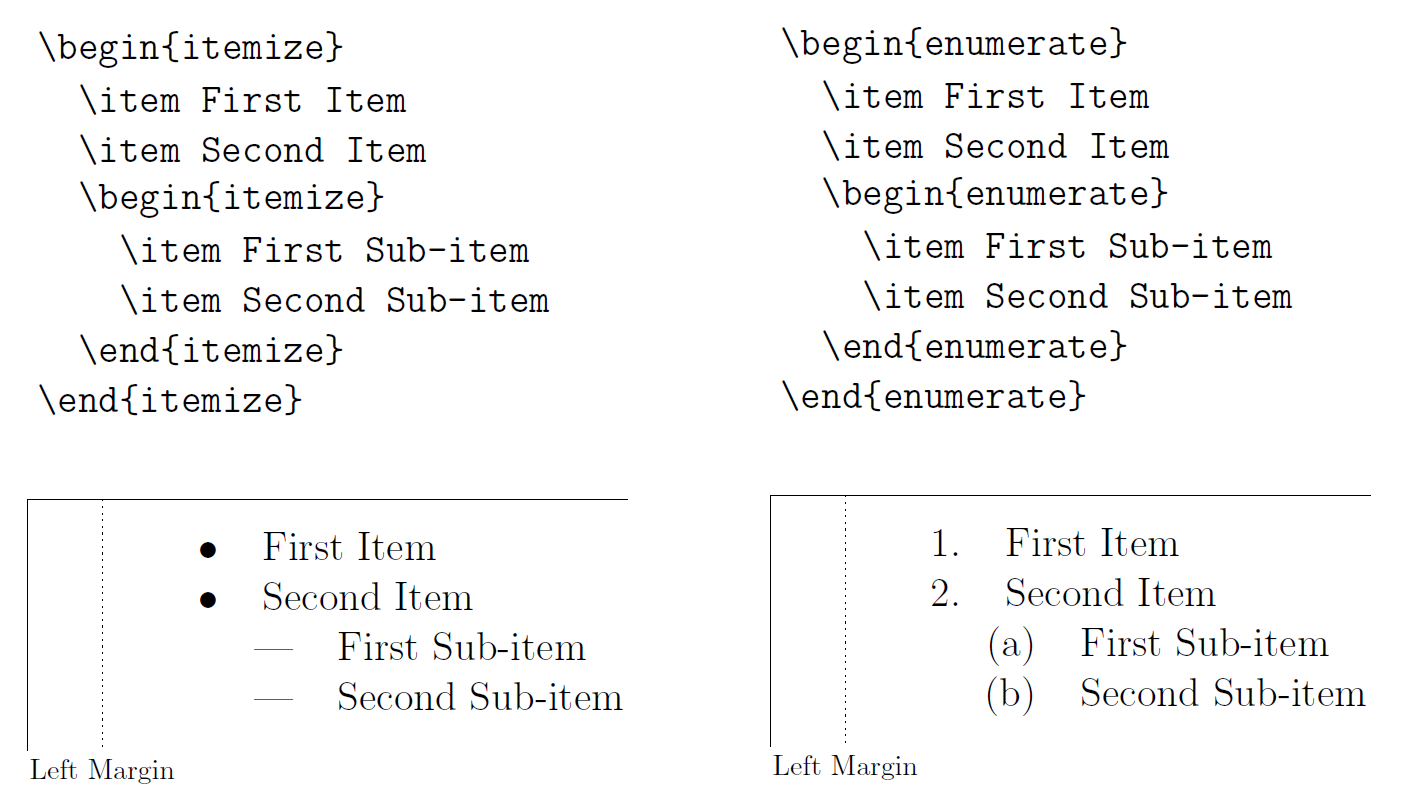
\includegraphics[scale=0.3]{figs/lists.png}
\end{center}
\end{frame}
%==============================================
\begin{frame}
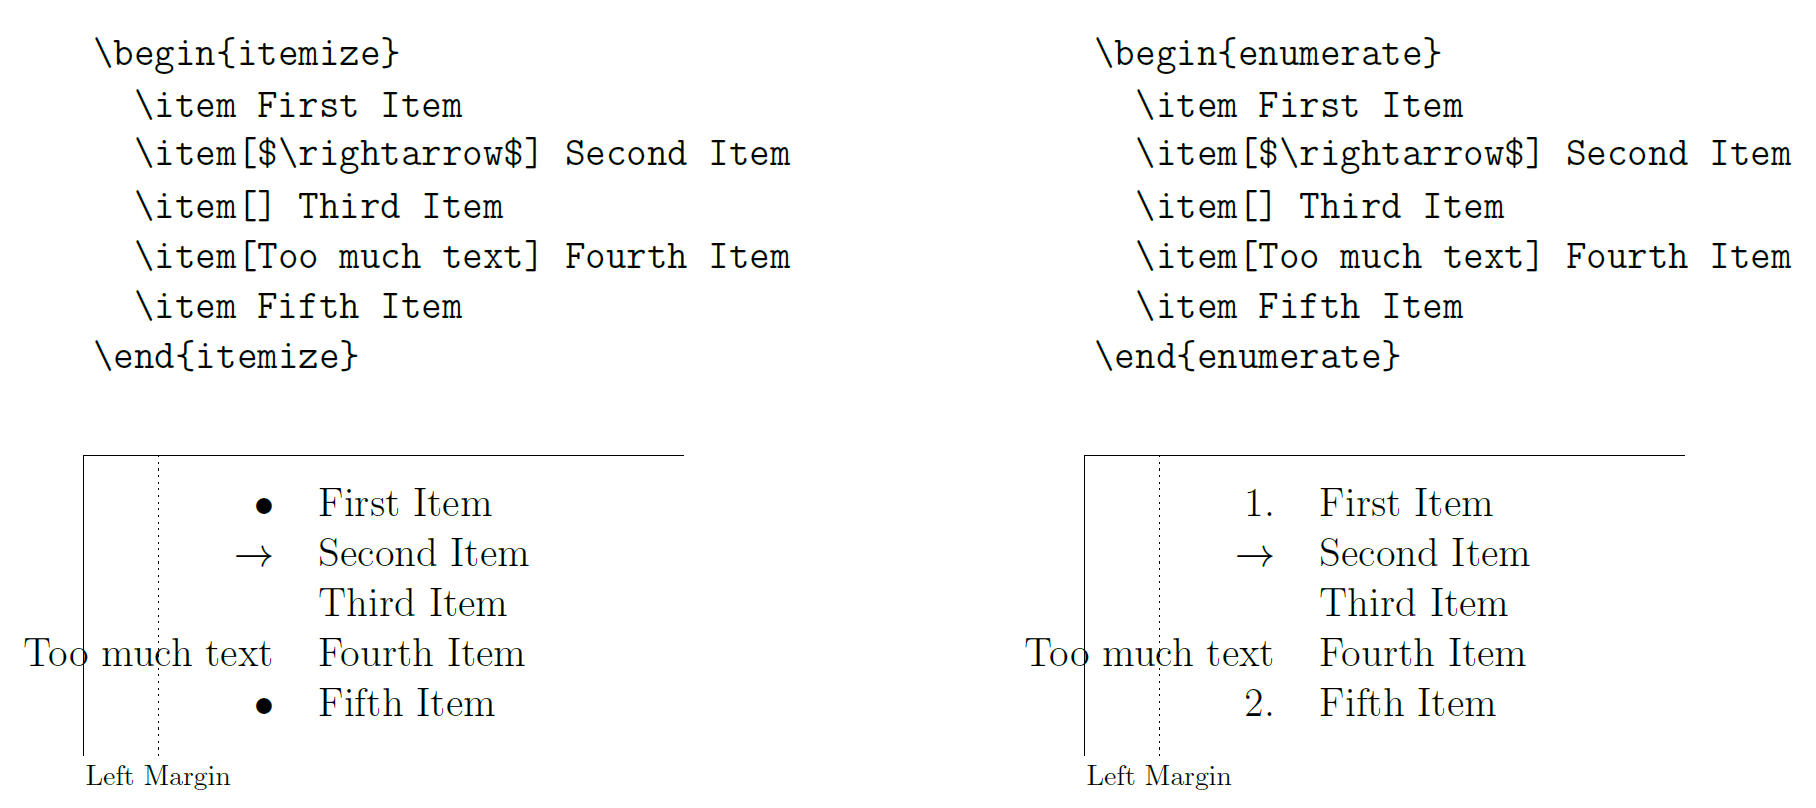
\includegraphics[width=11cm]{figs/lists2.png}
\end{frame}
%==============================================
\begin{frame}{الصيغ الرياضية و الرموز}
\begin{center}
    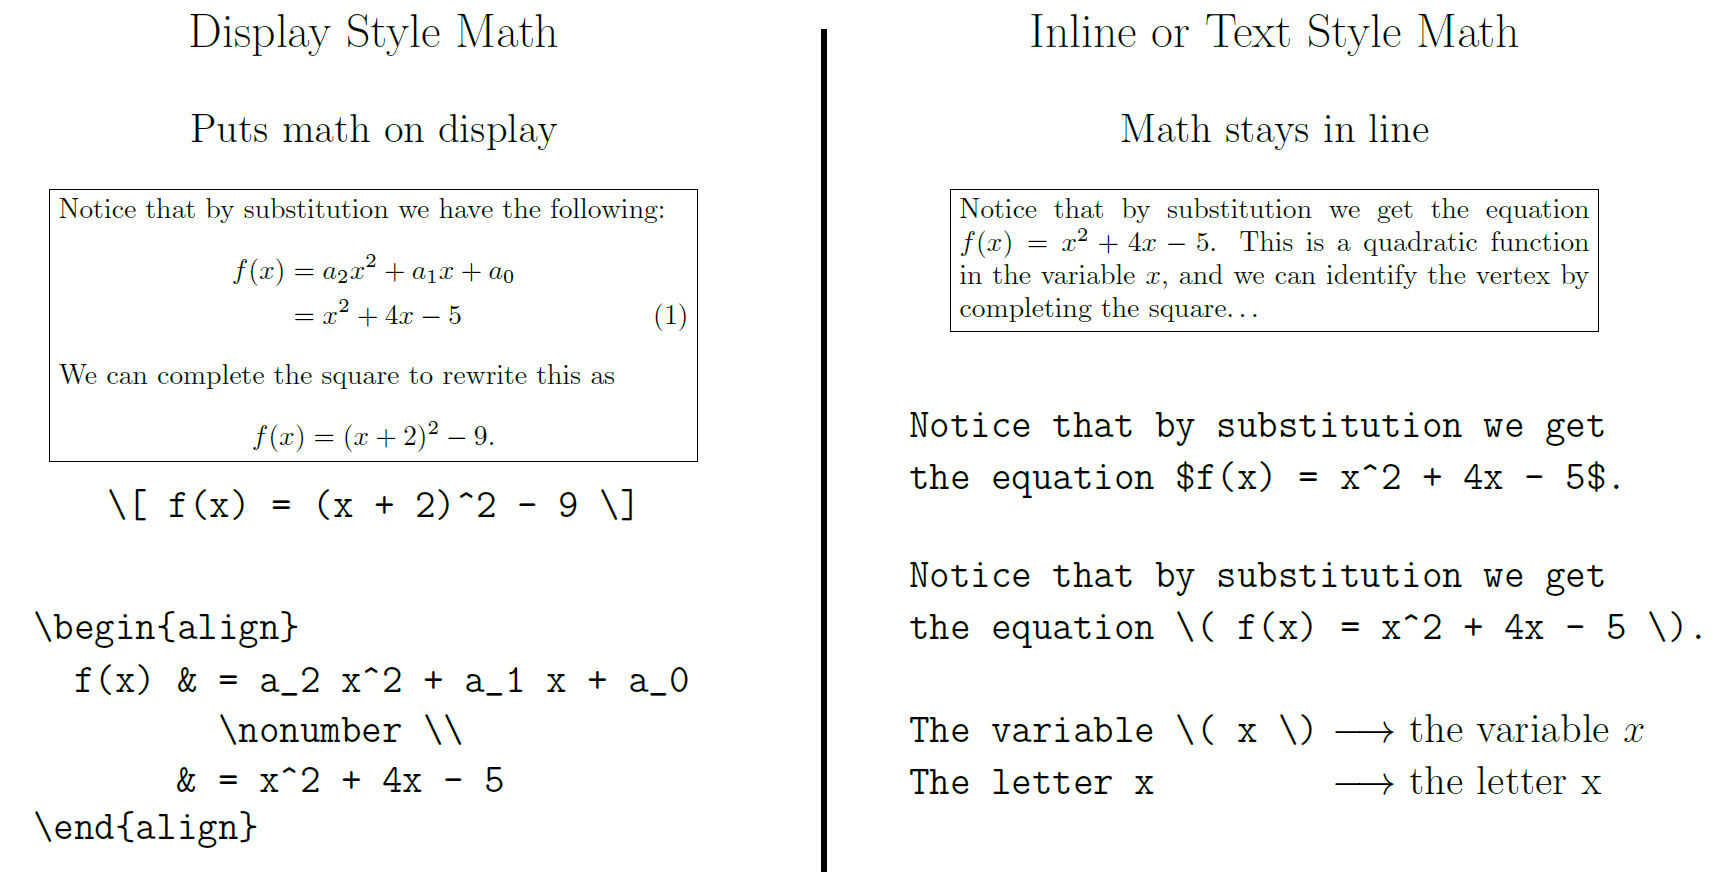
\includegraphics[width=11.5cm]{figs/math1.png}
\end{center}
\end{frame}
%==============================================
%\begin{frame}{الصيغ الرياضية و الرموز}
%\begin{center}
%    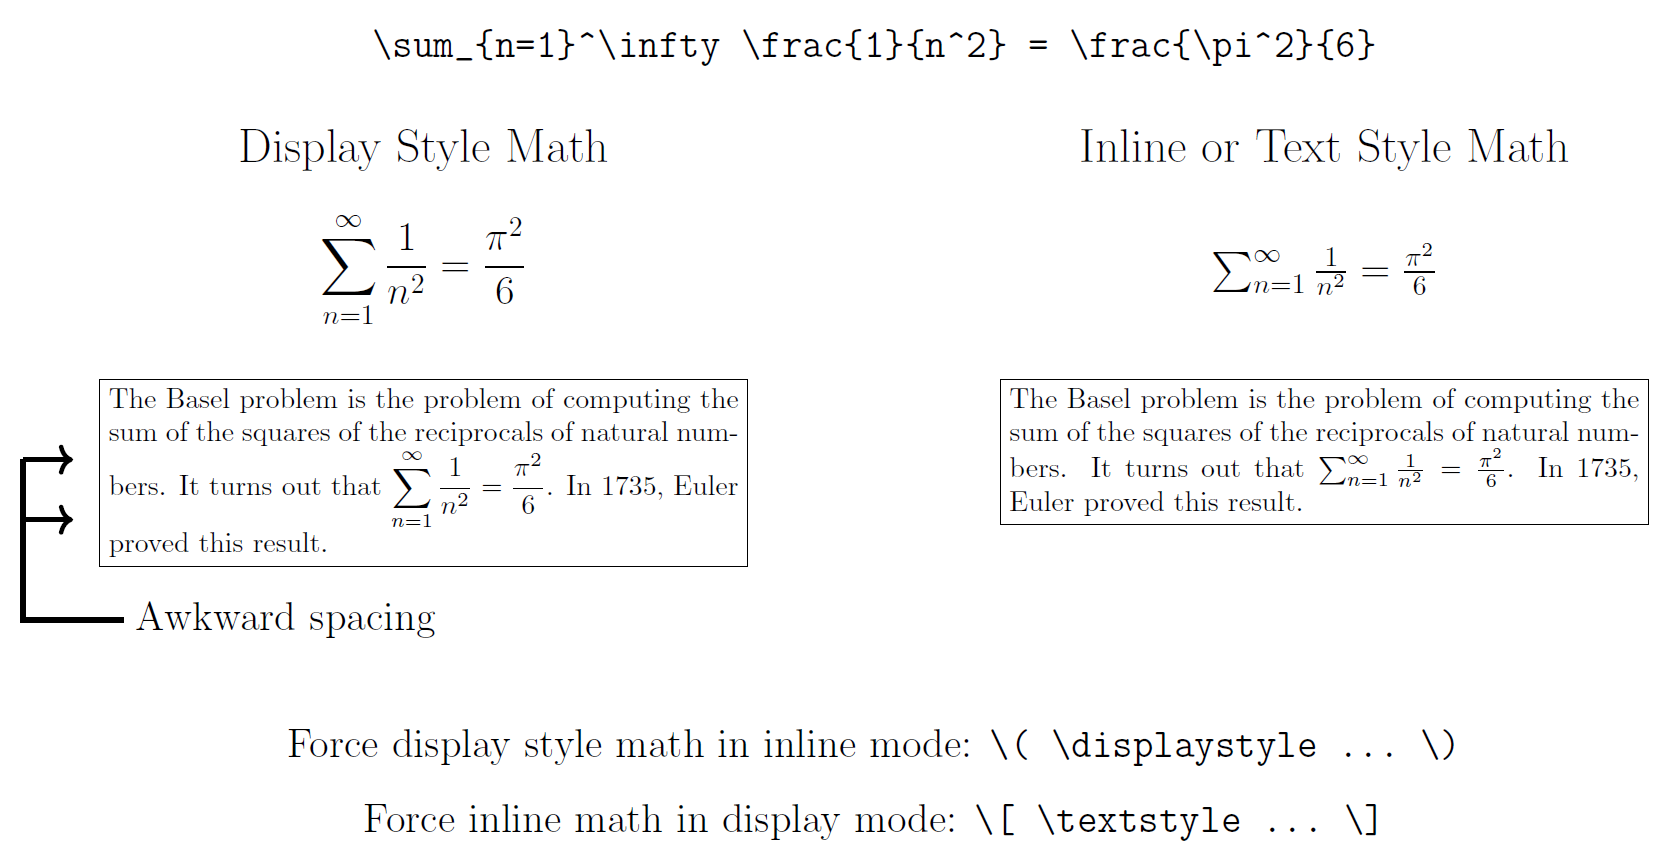
\includegraphics[width=11.5cm]{figs/math2.png}
%\end{center}
%\end{frame}
%==============================================
%\begin{frame}{الصيغ الرياضية و الرموز}
%\begin{center}
%    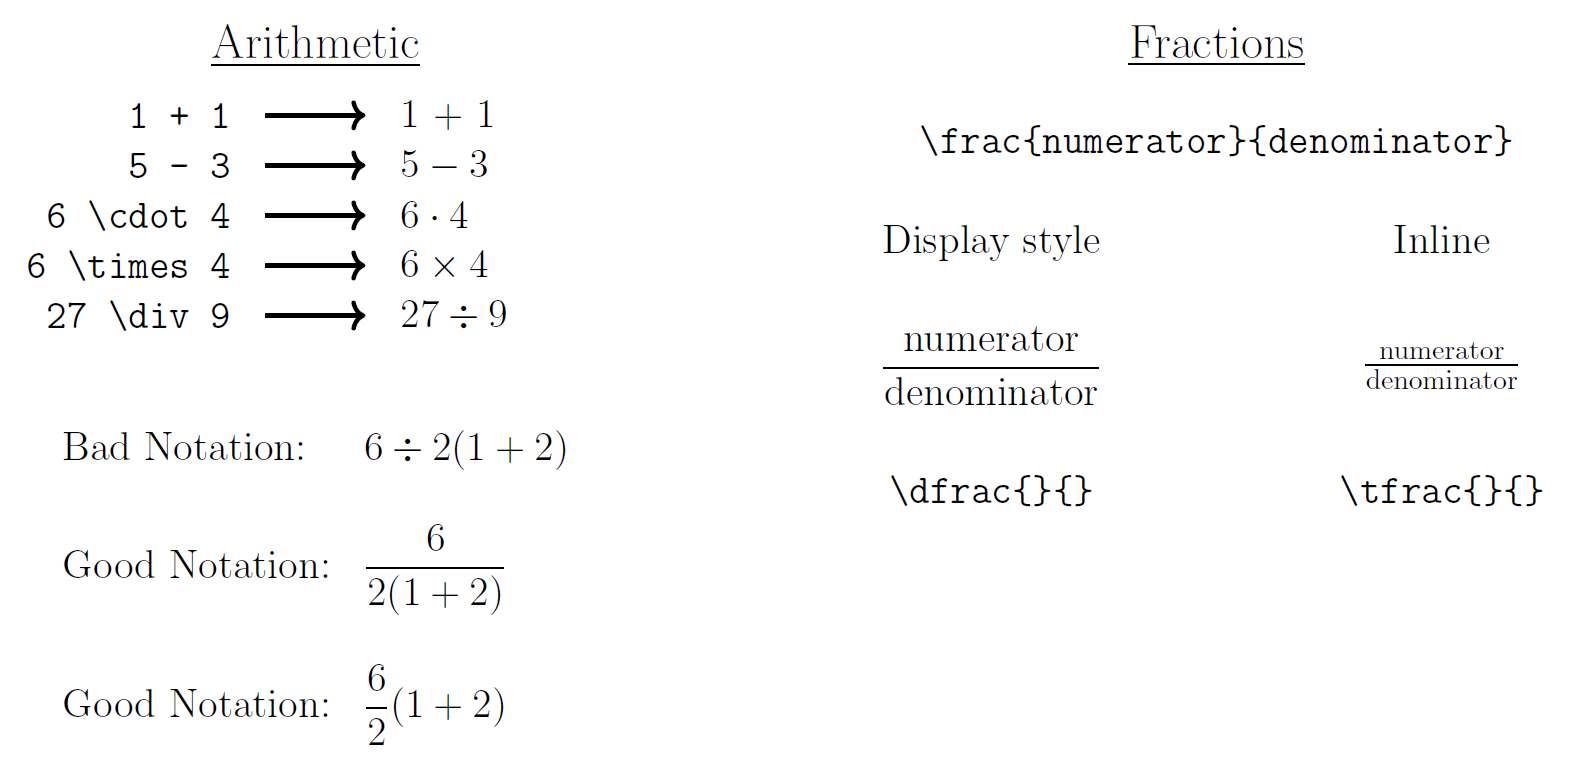
\includegraphics[width=11.5cm]{figs/math4.png}
%\end{center}
%\end{frame}
%==============================================
%\begin{frame}{الصيغ الرياضية و الرموز}
%\begin{center}
%    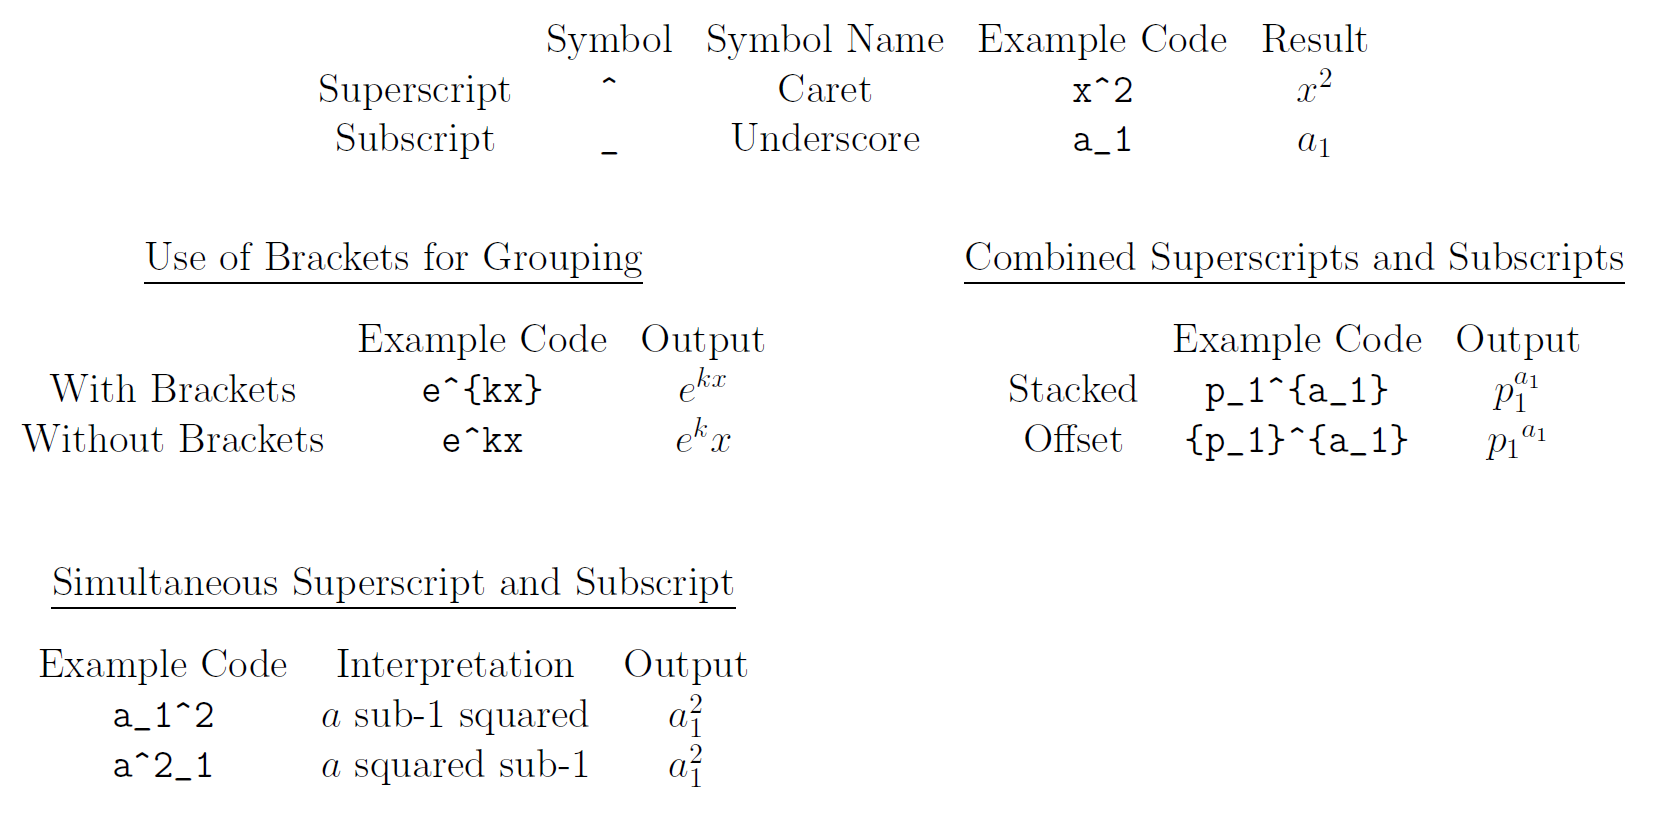
\includegraphics[width=11.5cm]{figs/math6.png}
%\end{center}
%\end{frame}
%==============================================
\begin{frame}{ادراج الصور}
 %\rtx{https://www1.cmc.edu/pages/faculty/aaksoy/latex/latexthree.html}
\bc
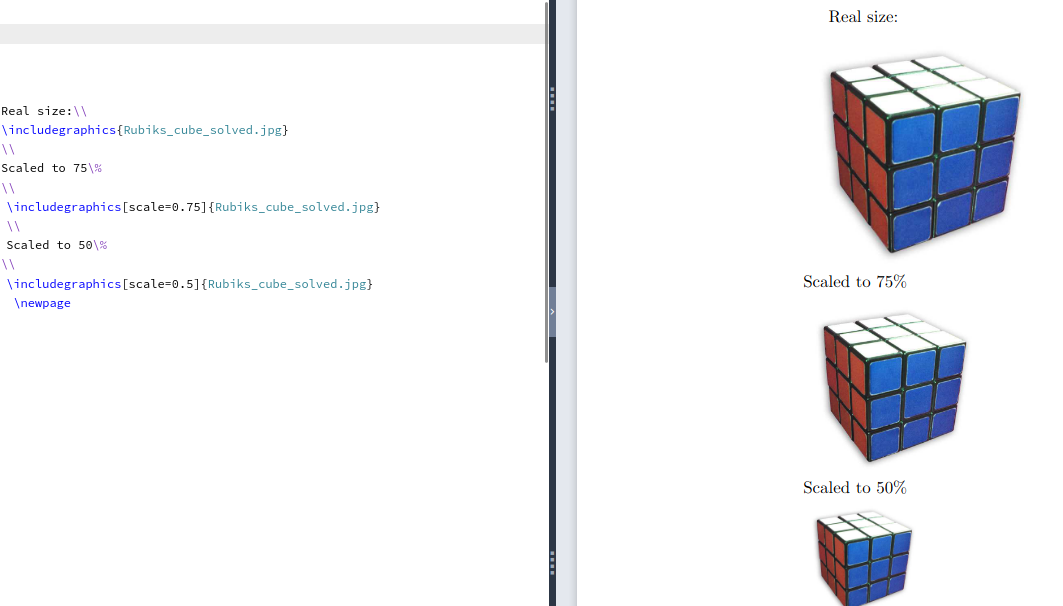
\includegraphics[scale=0.3]{figs/pics1.png}
\ec
\end{frame}

%==============================================
% \begin{frame}{ادراج الصور}
 %\rtx{https://www1.cmc.edu/pages/faculty/aaksoy/latex/latexthree.html}
%\bc
%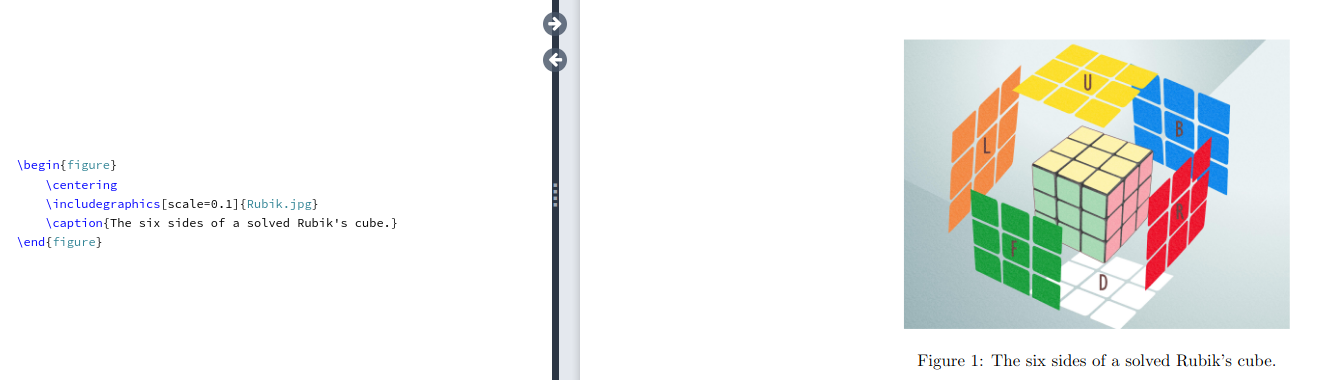
\includegraphics[scale=0.25]{figs/pics2.png}
%\ec
%\end{frame}
%==============================================
\section{روابط مفيدة}
\begin{frame}{روابط مفيدة}
\begin{itemize}\RTListe
    \item\href{https://www.overleaf.com/learn/latex/Tutorials}{تيتوريالات و تمارين  على الموقع الرسمي  ل Overleaf}
    \vspace{0.5cm}
\item \href{https://en.wikipedia.org/wiki/List_of_mathematical_symbols_by_subject}{قائمة الرموز الرياضية حسب الموضوع}
\vspace{0.5cm}
\item \href{https://tex.stackexchange.com/}{موقع أسئلة وأجوبة لمستخدمي \TeX{} و \LaTeX{} }
\vspace{0.5cm}
\item \href{https://www.latex-project.org/help/books/}{كتب مفيدة}
\vspace{0.5cm}
\item \href{https://github.com/Moh-Maher/LaTeX-Typesetting}{رابط مباشر لملفات اللاتك الخاصة بهذ العرض}
\end{itemize}
\end{frame}

\end{document}